\documentclass[12pt]{article}
\usepackage{amsmath,amsfonts,amssymb}
\usepackage{graphicx}
\usepackage{hyperref}
\usepackage{authblk}
\usepackage[backend=biber]{biblatex}
\newtheorem{lemma}{Lemma}
\newtheorem{definition}{Definition}
\newtheorem{remark}{Remark}

\addbibresource{../references.bib}
\title{The Abstract Universe: A Minimal Informational Model of Reality}
\author{Juha Meskanen}
\date{July 2025}

\begin{document}

\maketitle

\begin{abstract}
    Building on our earlier proposal that the universe is fundamentally informational in nature,
    we propose a radically minimalist foundation for physics based on information only.
    The framework assumes no primitive physical substrate—no predefined spacetime, particles, or fields.
    Everything we observe, from matter to consciousness, is modeled as an emergent structure within a fundamentally informational universe.
\end{abstract}



\section{Observational Assumptions}

We start with four observational assumptions. These are empirically grounded regularities,
each supported by real-world examples or established computational models. They are deliberately
minimal and falsifiable. If any one of them were shown to be invalid, the conclusions of this theory would not follow.

\paragraph{Assumption 1: Memory Requires Information Preservation}

\emph{Any observer capable of memory must preserve information across internal states.}

\vspace{0.2em}
This reflects the basic fact that for an observer to retain and recall experiences, the observer's internal structure must persist and encode past information. This is true of human cognition, digital memory systems, and even simple biological organisms.

\emph{Implication:} There must exist a substrate—physical or virtual—that allows for stateful information retention across time.

---

\paragraph{Assumption 2: Information Can Be Represented by Bitstrings}

\emph{Any physical or cognitive state can be encoded as a finite sequence of discrete symbols (e.g., a bitstring).}

\vspace{0.2em}
This is not a commitment to digital physics, but an acknowledgment that, for the purposes of modeling and communication, all observable phenomena can be encoded discretely. DNA, brain states, and digital computers all support this view.

\emph{Implication:} For modeling purposes, we can assume a discrete representation of observers and systems without loss of generality.

---

\paragraph{Assumption 3: Computation Is a Physical Process}

\emph{All physically realizable processes can be modeled as computation.}

\vspace{0.2em}
This aligns with the Church-Turing-Deutsch thesis and is broadly supported by the success of computational models in physics and biology. This assumption is empirical: no known physical process has been shown to lie outside computational modeling.

\emph{Implication:} Any observer or system can be described as a sequence of computational state transitions—an execution trace.

---

\paragraph{Assumption 4: Causality is Represented by Ordered States}

\emph{Causal structure corresponds to the sequential ordering of informational states.}

\vspace{0.2em}
In practice, we observe events as sequences: perception follows stimulus, memory encodes before retrieval, and measurements yield outputs after inputs. We assume that causality is experienced as an ordering of state transitions, not imposed externally.

\emph{Implication:} Time and causality are not primitive; they are emergent from the order in which informational states are experienced.

---

Together, these four assumptions provide the foundation for the theory that follows. They assert that memory, representation, computation, and causality are all observable features of physical reality. No metaphysical entities are required.

All structure, from particles to consciousness, arises from the combinatorics of information patterns and their observer-relative interpretations.





\section*{The Observer Prevalence Principle}

Let $n$ be a fixed number of bits. Let $\mathcal{U}_n = \{0,1\}^n$ denote the set of all $2^n$ binary strings, interpreted as candidate universes. Let $\mathcal{O}_n = \{0,1\}^n$ denote the same set, interpreted as candidate observers.

Define a \textbf{compatibility function}
\[
    \mathrm{Compat}: \mathcal{O}_n \times \mathcal{U}_n \rightarrow \{0,1\}
\]
such that $\mathrm{Compat}(o, u) = 1$ if observer $o$ can exist within universe $u$ under a chosen observer model (e.g., memory encoding, trajectory embedding, structural motif match), and 0 otherwise.

\begin{definition}[Observer Prevalence Principle]
    The \emph{subjective probability} that a given observer $o \in \mathcal{O}_n$ experiences a particular universe $u \in \mathcal{U}_n$ is proportional to the number of universes compatible with $o$:
    \[
        \Pr(u \mid o) \propto \mathrm{Compat}(o, u).
    \]
    Equivalently, the most probable universe an observer experiences is the one maximizing the number of observer-compatible instances:
    \[
        u^* = \arg\max_{u \in \mathcal{U}_n} \sum_{o \in \mathcal{O}_n} \mathrm{Compat}(o, u).
    \]
\end{definition}

This principle implies that the observed universe is biased toward configurations that support the maximal number of observers isomorphic to the subject, leading to emergent regularities (e.g., smooth physical laws, coherent time evolution) that favor observer persistence.

\begin{remark}
    The special case where an observer $o$ is identical to a universe $u$ (i.e., $o = u$ and $\mathrm{Compat}(o, u) = 1$ trivially) defines a fixed point of maximal internal consistency. This limiting case represents an informational singularity—an observer-universe with no internal entropy or external reference.
\end{remark}



\section{Framework and Definitions}

Let $B$ denote the total number of bits used to describe a universe. We define:

\begin{itemize}
    \item $\mathcal{U}_B$: the set of all possible universes composed of bitstrings of length $B$, partitioned into frames $f_i$ representing temporal slices.
    \item $O = \{o_1, o_2, \ldots, o_n\}$: a sequence of bitstrings representing the observer's memory and state across subjective time.
\end{itemize}

\subsection{Observer-Centric Universe Construction Principle (OCUCP)}


An observer exists in those universes $U \in \mathcal{U}_B$ where their memory patterns $o_i$ are statistically embedded within the universe frames $f_i$. The ontology is relational: observer existence is defined probabilistically by structural compatibility rather than by deterministic selection.


\subsection{Observer Contuinity Lemma (OCL)}

Let $O = \{o_1, o_2, \ldots, o_n\}$ be an observer trajectory, and $F = \{f_1, f_2, \ldots, f_n\}$ a candidate sequence of universe frames. Then, the observer can only \emph{remember} or \emph{experience} $F$ if:

\[
    \exists\ \epsilon > 0\ \text{ such that }\ \text{Similarity}(o_i, f_i) \ge \epsilon\ \text{ for all } i.
\]

In other words, the observer's internal structure must sufficiently overlap with the universe frames for continuity and memory to be possible. Memory is defined as structural self-similarity over time, not as causal flow.

\subsection{Similarity Metric and Observer Survival}

We define a similarity function $\text{Sim}(a, b)$ between two bitstrings. An observer $O$ survives a frame transition $o_i \to o_{i+1}$ only if $\text{Sim}(o_i, o_{i+1}) \ge \delta$ for some threshold $\delta$. This defines a selection criterion over possible trajectories.

\section{Compression and the Wavefunction}

We propose a new interpretation of the quantum wavefunction grounded in the logic of observer survival through compression.

\subsection{Compression Bias Principle (CBP)}

Let $C(F)$ denote the compressed length of a sequence of universe frames $F = \{f_1, \ldots, f_n\}$. Then, the number of observers that can embed within $F$ is inversely correlated with $C(F)$.

That is, smooth, regular, and compressible universes support more observers, simply because more observer trajectories can be accommodated within the same limited bit budget. Consequently, the universe we find ourselves in is likely to be highly compressible.

\subsection{Wavefunction as Compressed Continuation}

An observer’s internal model probabilistically extrapolates future frames by identifying structural regularities and compression patterns. This naturally leads to multiple possible continuations weighted by their compressibility, forming an informational “superposition” rather than a deterministic path.

\begin{itemize}
    \item The observer contains past states $\{o_1, \ldots, o_t\}$.
    \item It extrapolates possible futures $o_{t+1}, \ldots, o_{t+k}$ using pattern completion.
    \item If the compression basis is Fourier/sine-based, extrapolation leads to smooth predictions.
    \item Multiple continuations are possible, forming a "superposition" within the observer's internal model.
\end{itemize}

Interference arises when extrapolated continuations reuse shared substrings. Thus, quantum phenomena emerge not from physical superposition, but from ambiguous extrapolations under compression logic. This model views the wavefunction as an efficient coding scheme, not as a physical entity.

\section{Entanglement and Shared Memory}

Entanglement is modeled as mutual constraint between observer subcomponents. If two observer bitstrings $A$ and $B$ share internal fragments and exist within a common universe $U$, then the observer can only survive in frames that preserve both. This shared structure constrains joint probabilities, introducing entanglement.


\section{Simulation}

We present a simulation program implementing the above described formal model as Python program.

Given observer, as bitstring evolving in time, the program find the most likely spacetime configuration from the observer's point of view.

The user interface to the program allows the observer to be defined conveniently as a
2D dimensional shape, where X dimension corresponds to space and Y corresponds to time.
Program converts the observer to wavefunction.

\begin{figure}[h!]
    \centering
    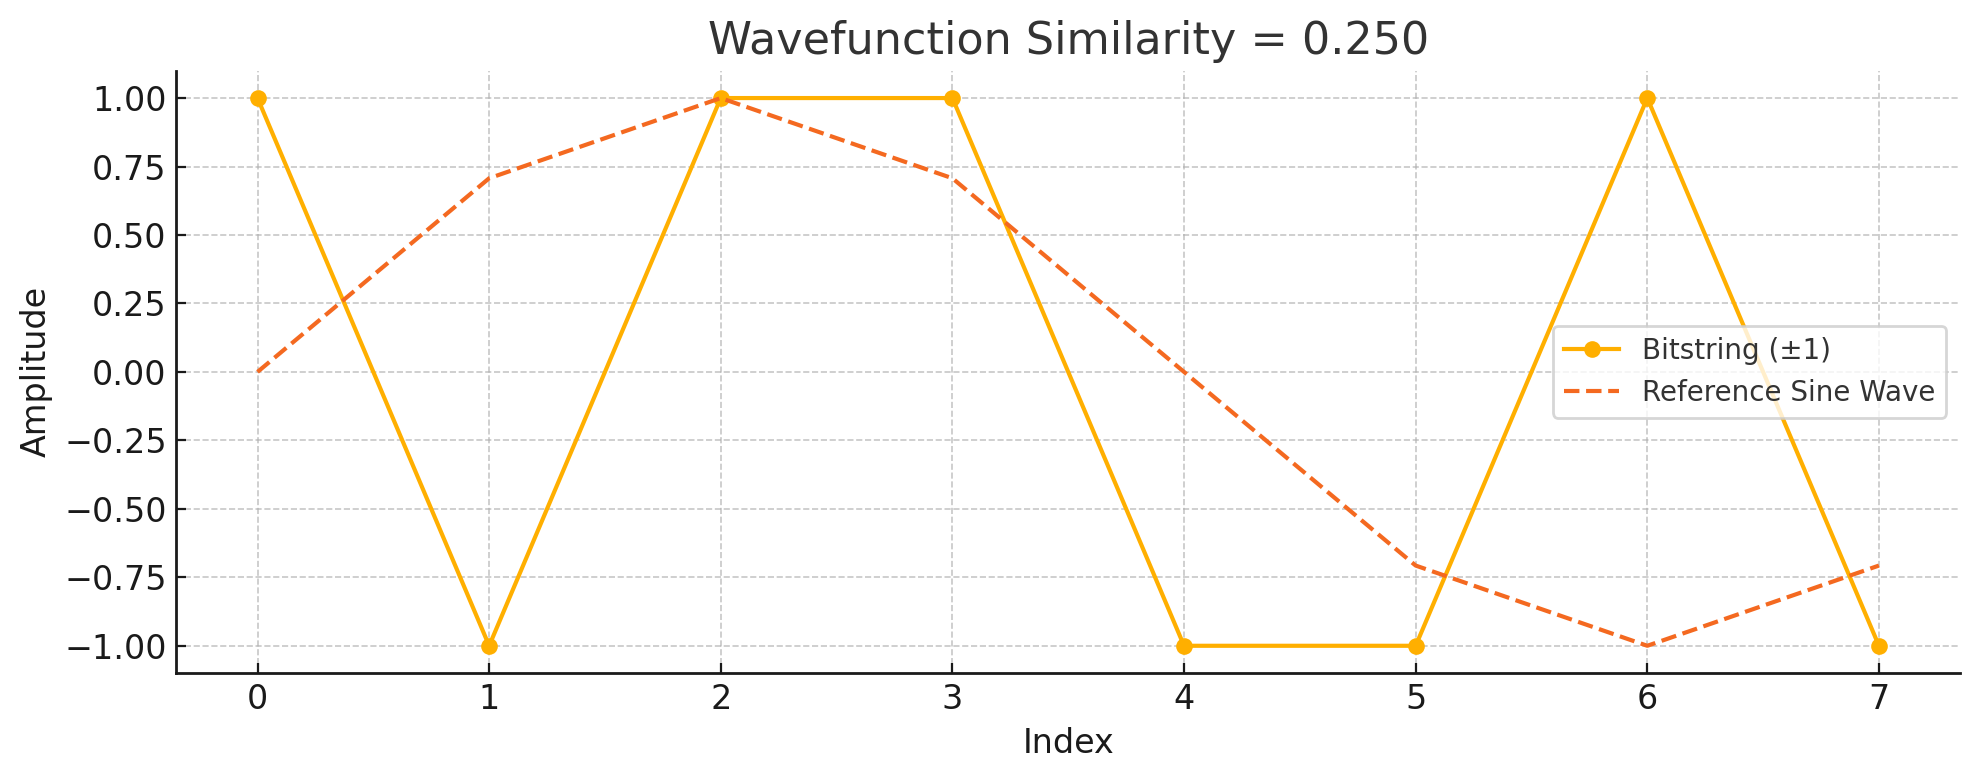
\includegraphics[width=1.0\textwidth]{figures/wavefunction_similarity.png}
    \caption{The wavefunction representation of the discrete observer.}
    \label{fig:wavefunction_similarity}
\end{figure}


Finite **Fourier components** is used for compressing data.
This naturally leads to  quantum-probability interpretation of observer presence via wavefunction overlap.

\subsection{Compression, Fourier, and Bayesian Filtering}

\begin{itemize}
    \item **Observer**: A predefined binary matrix (e.g., a circle) representing a structure in spacetime.
    \item **Universe**: A 2D spacetime information field constructed using a limited set of sine/cosine waves (compressed Fourier basis).
    \item **Similarity Matching** correlation of observer pattern with continuous field — interpreted as a **probability amplitude**.
    \item **Selection**: From multiple generated universes, the simulation selects the one where the observer appears most clearly.
\end{itemize}

\subsection{Compression and Probability}

\begin{itemize}
    \item Compression is equivalent to probability: more compressible states are more likely under an algorithmic prior (Solomonoff).
    \item Fourier modes serve as a natural basis for compressible spacetimes.
    \item Limiting to a sparse Fourier spectrum implies we are only sampling from the most probable universes.
\end{itemize}

\subsection{Bayesian Filtering Analogy}


\begin{itemize}
    \item **Hypothesis space** = All possible spacetime bitstrings
    \item **Prior** = Simpler (more compressible) bitstrings are more likely (Fourier-limited)
    \item **Likelihood** = Observer pattern matches (how often the observer appears)
    \item **Posterior** $\propto$ Prior $\times$ Likelihood $\rightarrow$ Highest when a compressible spacetime contains a dense observer
\end{itemize}

\subsection{Results}

The program creates four different plots to visualize the universe that best implements the specified observer.

\begin{itemize}
    \item **Wavefunctions** emerge naturally from high-compression bitstring universes.
    \item **Interference** arises as the detection mechanism for observer motifs.
    \item **Physics** is recast as a filtering process where informational constraints select for structured realities.
\end{itemize}

From this perspective, quantum behavior, continuity, and even time are statistical artifacts of optimal observer embedding in
compressible informational structures.

\begin{figure}[h!]
    \centering
    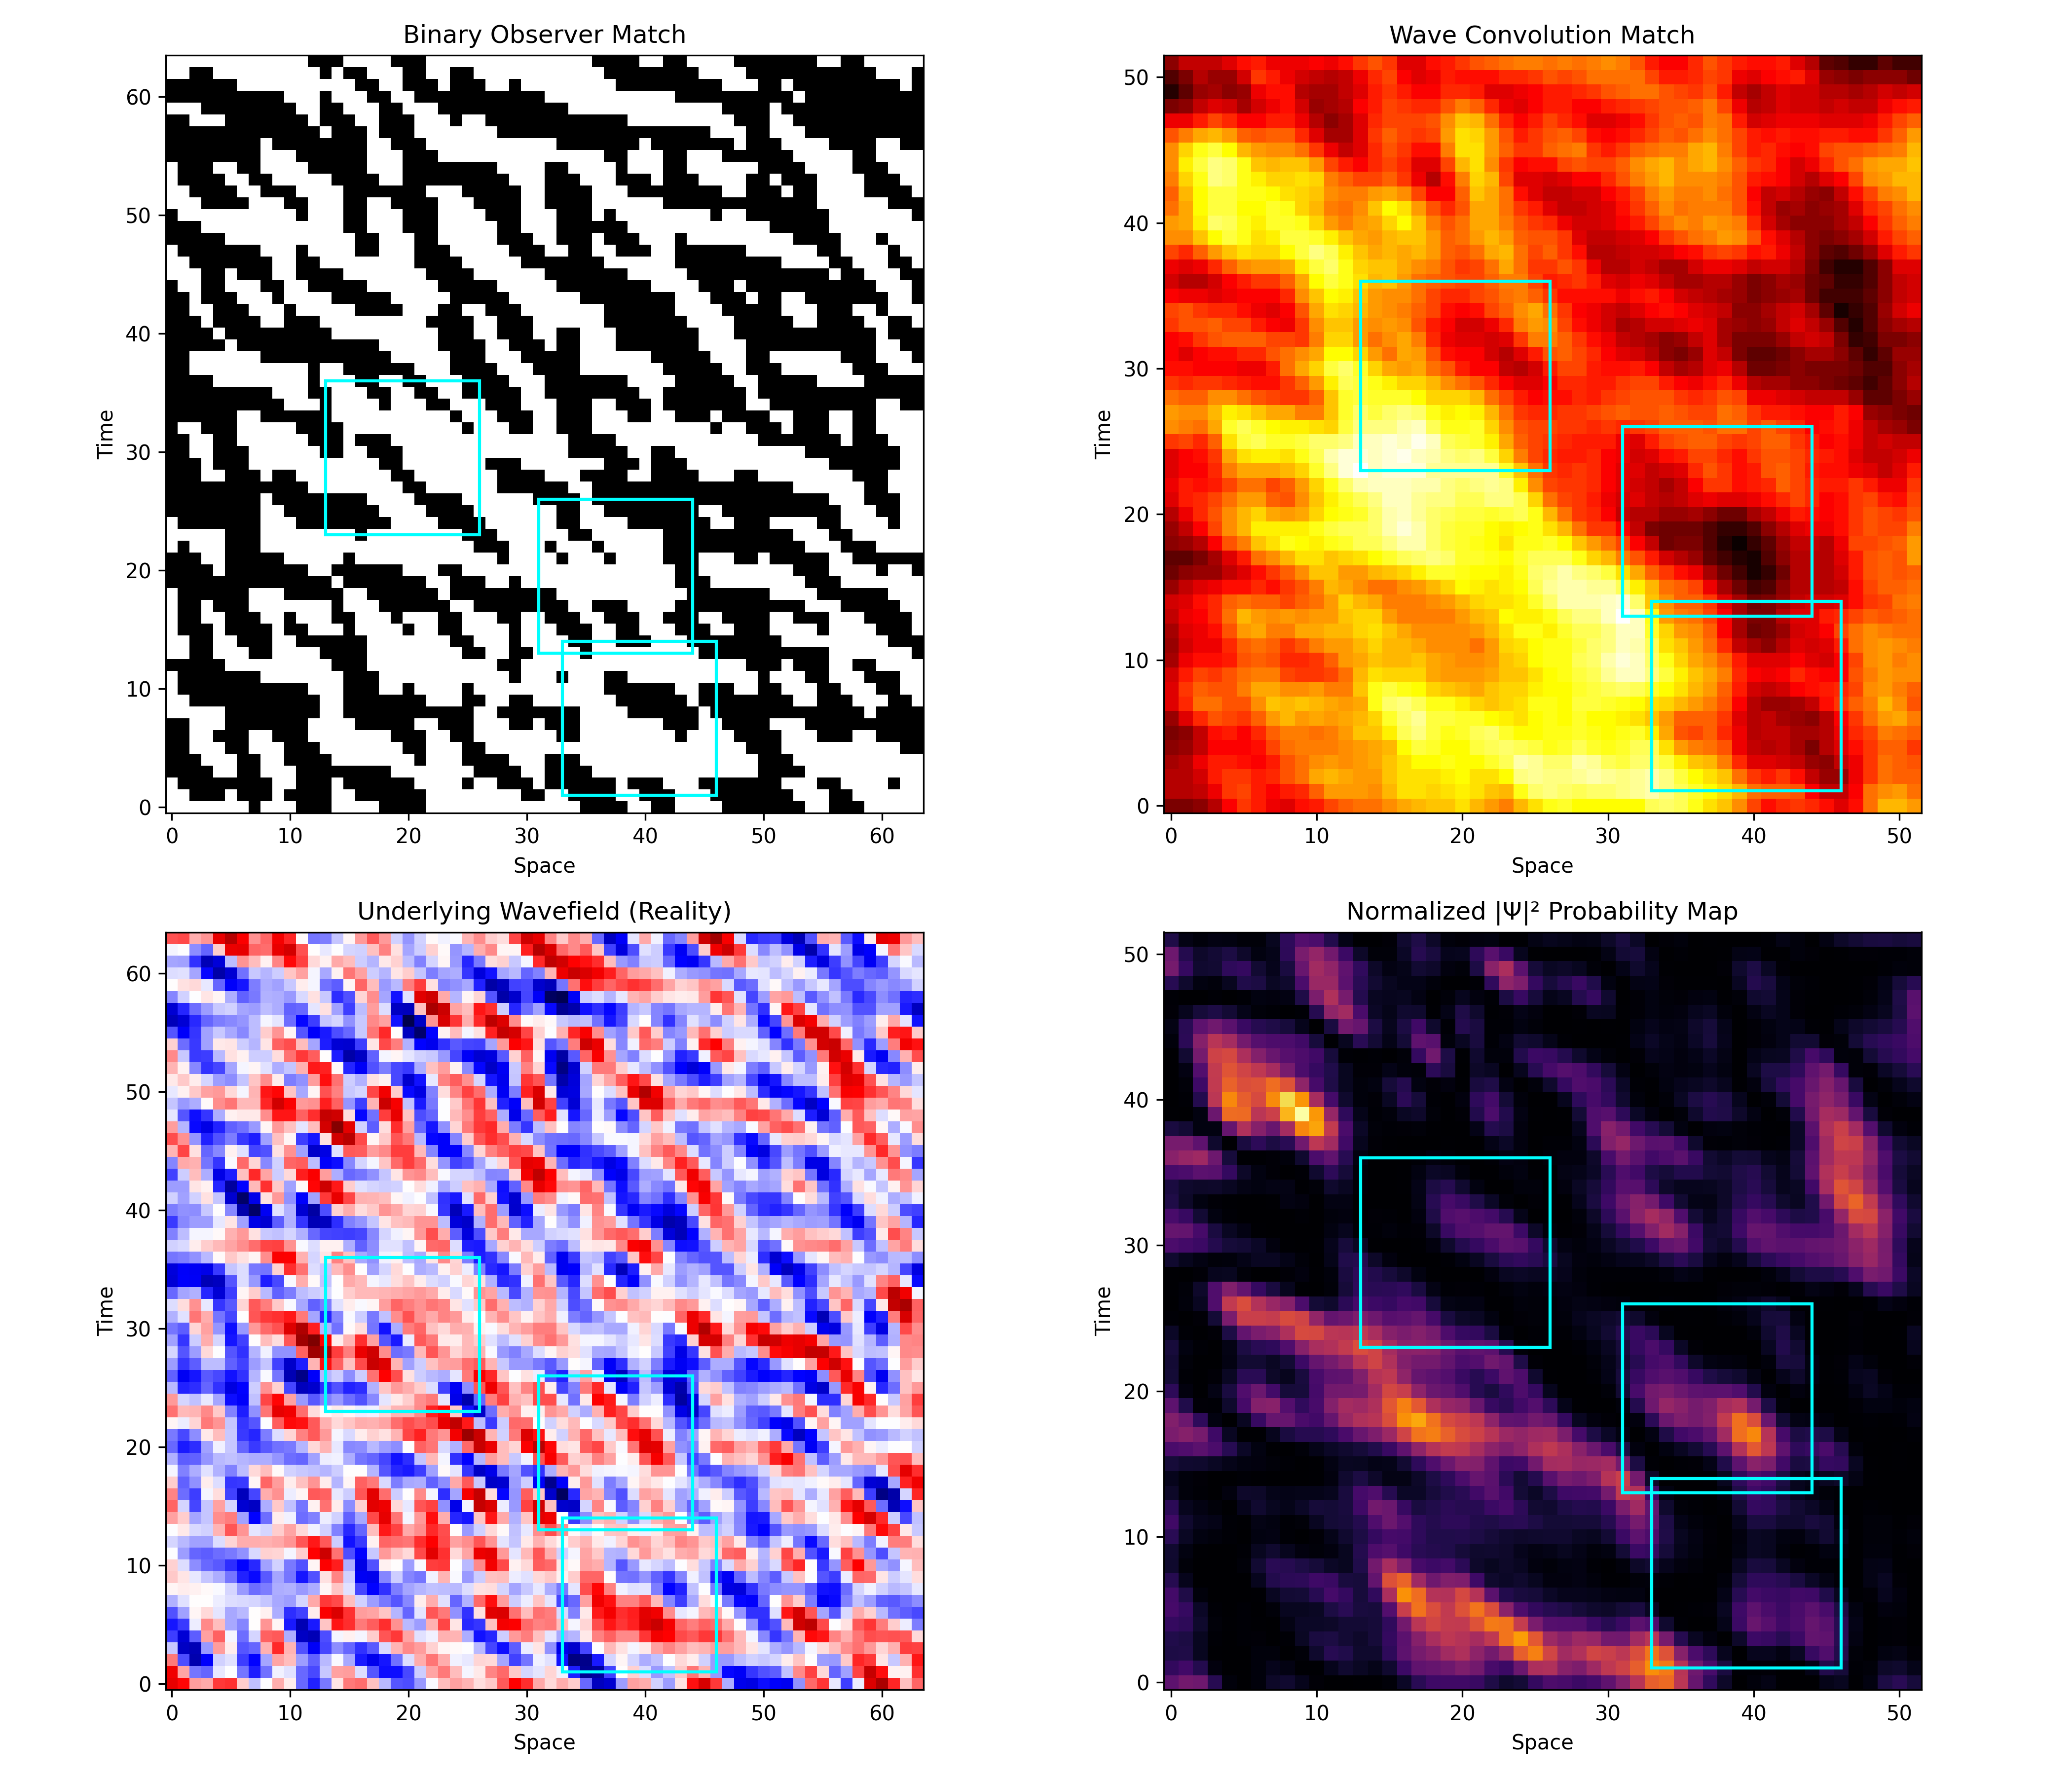
\includegraphics[width=1.0\textwidth]{figures/observer_wave_evolution.png}
    \caption{Four heatmaps visualizing observer wave evolution in the spacetime. }
    \label{fig:observer_wave_evolution}
\end{figure}

Past is those worlds the observer has high similarity. Future is those worlds that the observer has no shared sub-sets, but which the observer can "predict" by extrapolating with the wave function.

\begin{figure}[h!]
    \centering
    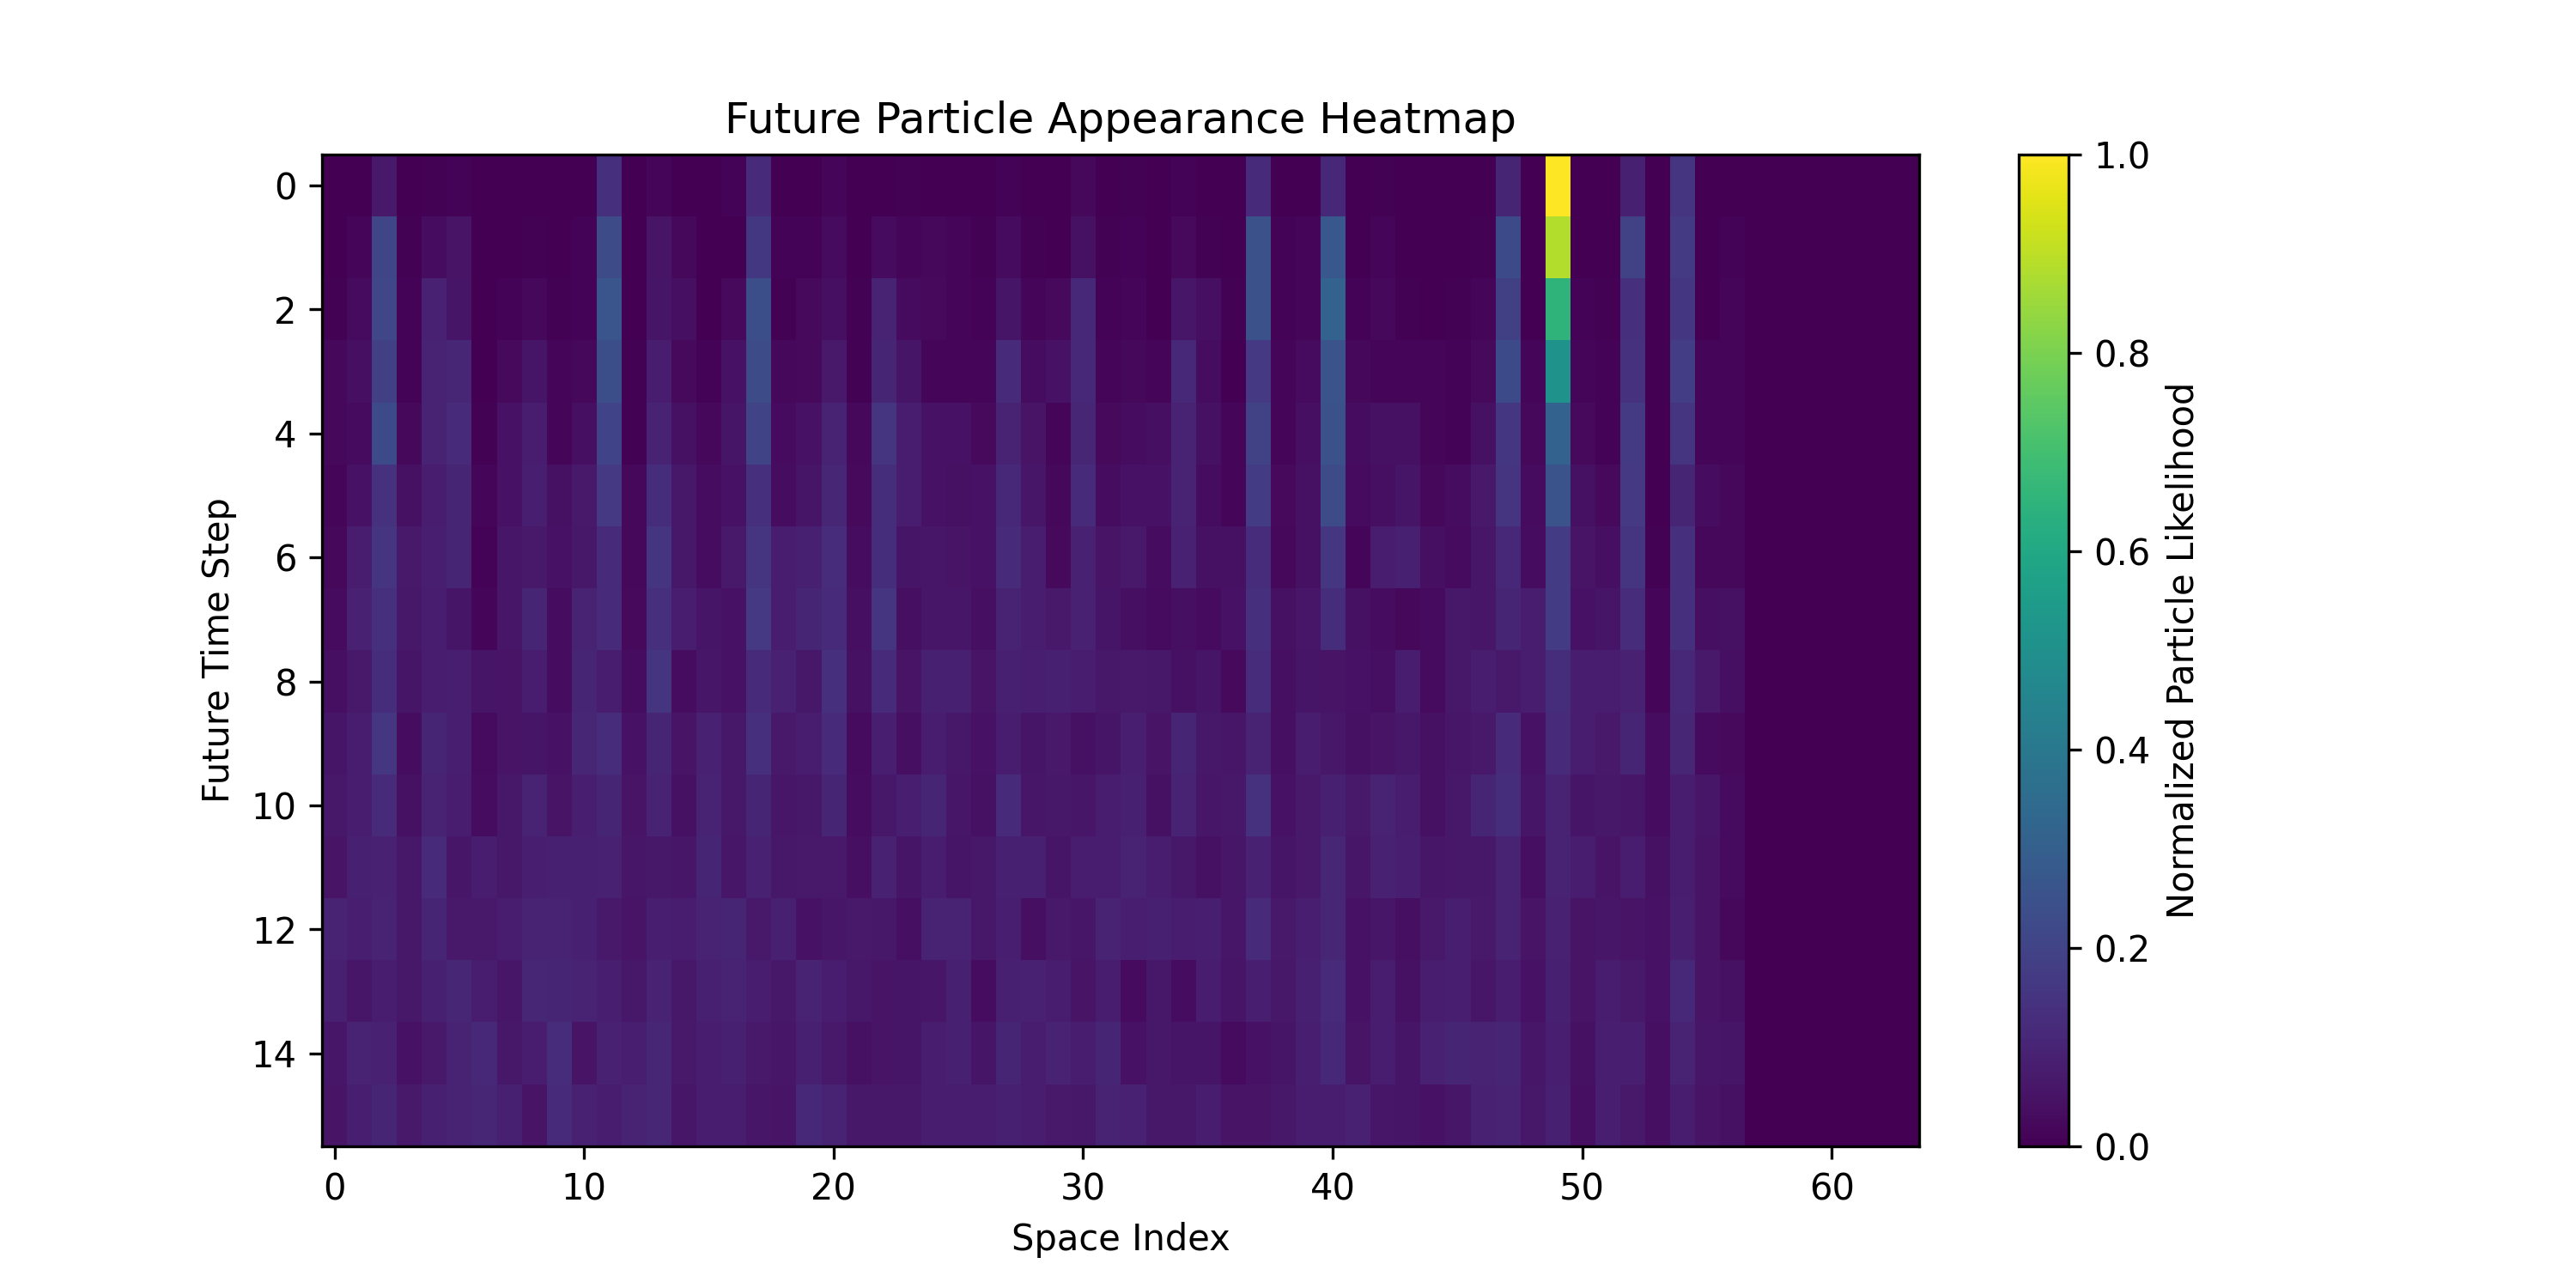
\includegraphics[width=1.0\textwidth]{figures/future_particle_heatmap.png}
    \caption{Heatmap visualizing possible future worlds. The image shows the density of particle trajectories in the future, indicating where observers or particles are likely to find consistent continuations. The future is not a single path but a set of probable continuations shaped by the observer's past. Predictability fades with distance from the current state as possible continuations proliferate. The user can not predict the future very far}
    \label{fig:future_particle_heatmap}
\end{figure}


The program is hosted at:
\[
    \texttt{http://github.com/juhakm/simulations/paper4/simulation.py}
\]

\section{Discussion and Implications}

In this framework, we reject the presumption that spacetime or particles are ontologically fundamental \cite{wheeler1990it} \citation{zuse1970calculating}.
Conventional notions of causality and dynamics are replaced in favor of a static informational ontology. There is no concept of interaction.

Universes are static informational structures, with observer experience arising from statistical compatibility between memory fragments and universe configurations, giving the user the illusion of "remembering" the past. The “future” corresponds to a distribution over possible continuations, weighted by compression-based likelihood, rather than a uniquely evolving timeline.

There is no fundamental substrate—only bitstrings and the observer's search for consistent continuations. Gravity, time, and quantum effects emerge as statistical preferences under this framework.


\section{Conclusion}

We have proposed a minimal, observer-centric framework in which bitstring universes are filtered by the internal structure of the observer. This model integrates and extends our previous work by showing that classical and quantum phenomena alike can emerge from a single informational substrate, using compression and structural similarity as guiding principles. Probability, persistence, and interference arise not from physical causes but from the combinatorics of observer-compatible paths through the space of possible bitstring universes.

\section{Future Work}

\begin{itemize}
    \item  Apply the theory to study the nature of blackhole singularities
    \item  Derive how expanding universe can emerge from information
    \item  Generalize to 4D spacetime for 3D geometric shapes.
    \item  Show how General Relativty arises from the Theory
    \item  Allow 3D observers to be modeled using 3D modeling software.
    \item  Evaluate entropy gradients and emergent fields.
\end{itemize}



\begin{thebibliography}{9}
    \bibitem{lloyd}
    Lloyd, S. (2006). \textit{Programming the Universe}. Knopf.

    \bibitem{bousso}
    Bousso, R. (2002). The holographic principle. \textit{Reviews of Modern Physics}, 74(3), 825.

    \bibitem{rovelli}
    Rovelli, C. (1996). Relational quantum mechanics. \textit{International Journal of Theoretical Physics}, 35(8), 1637–1678.

    \bibitem{tegmark}
    Tegmark, M. (2008). The mathematical universe. \textit{Foundations of Physics}, 38(2), 101–150.

    \bibitem{shannon}
    Shannon, C. E. (1948). A mathematical theory of communication. \textit{Bell System Technical Journal}, 27, 379–423, 623–656.
\end{thebibliography}

\end{document}
